\documentclass[UTF8]{ctexart}

\title{电子技术基础实验第十二周实验报告}

\author{王磊\quad2022012972}

\date{\today}

\usepackage{geometry}
\geometry{a4paper,scale=0.8}

\usepackage{graphicx}
\usepackage{subfigure}
\usepackage{float}

\usepackage{amsmath}

\usepackage{listings}
\usepackage{xcolor}
\usepackage{framed}
\usepackage{placeins}
\usepackage{siunitx}
\lstdefinestyle{verilogStyle}{
    language=verilog,
    basicstyle=\ttfamily,
    keywordstyle=\color{blue},
    commentstyle=\color{green},
    stringstyle=\color{red},
    numbers=left,
    numberstyle=\tiny\color{gray},
    breaklines=true,
    showstringspaces=false,
    columns = fixed,
    basewidth = 0.5em,
    captionpos=b,
}
\newcommand{\subsubsubsection}[1]{\paragraph{#1}\mbox{}\\}
\setcounter{secnumdepth}{4} % how many sectioning levels to assign numbers to
\setcounter{tocdepth}{4} % how many sectioning levels to show in ToC
%设置段落间距
\setlength{\parskip}{0.5em}
%令小标题左对齐
\CTEXsetup[format={\Large\bfseries}]{section}
%首行不缩进
\setlength{\parindent}{0pt}
\begin{document}
\maketitle
\section{task1}
\subsection{模块设计}
\subsubsection{24位正弦数据生成}
使用matlab生成用于初始化ROM的mif文件,其中存储了256个24位的正弦数据,代码如图\ref{fig:matlab_code}所示。
\begin{figure}[!ht]
    \centering
    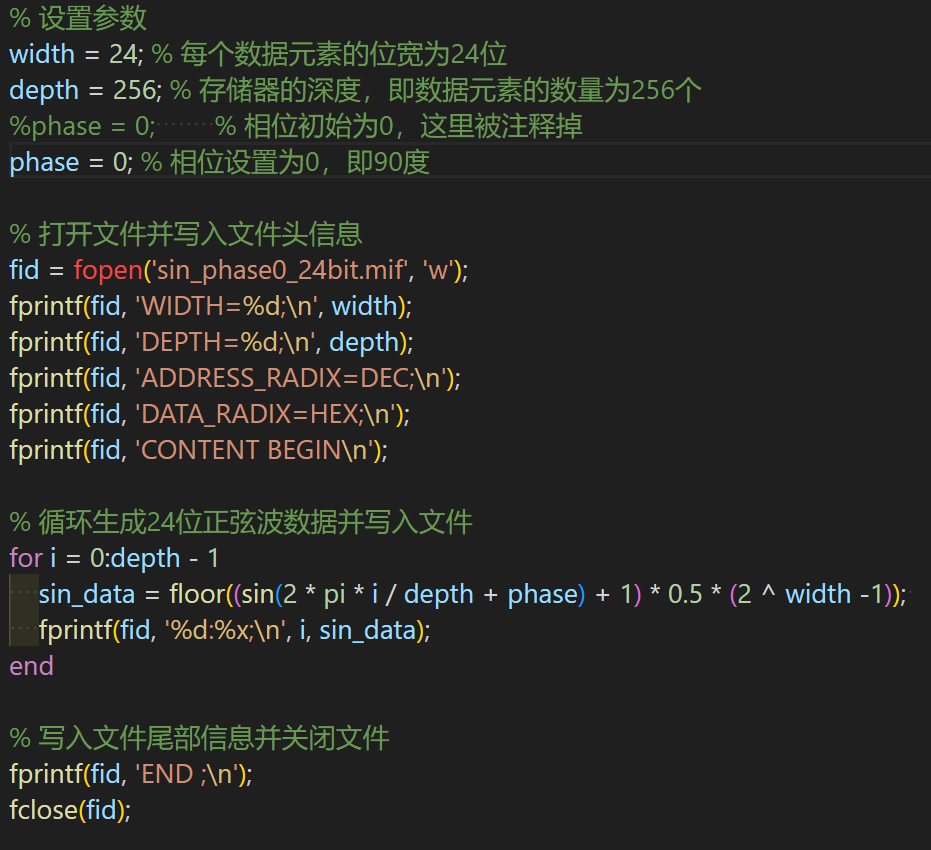
\includegraphics[width=0.8\textwidth]{matlab_code.png}
    \caption{matlab代码}
    \label{fig:matlab_code}
\end{figure}

生成的mif文件内容如图\ref{fig:mif}所示。
\begin{figure}[!ht]
    \centering
    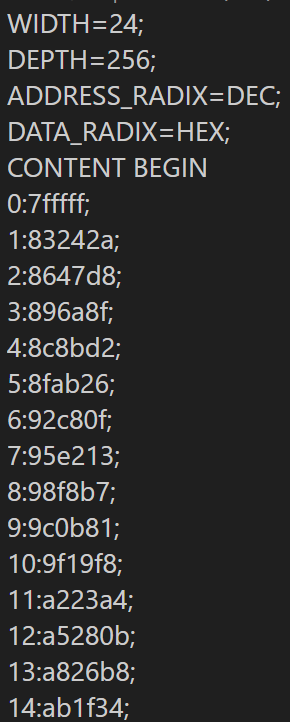
\includegraphics[width=0.4\textwidth]{mif.png}
    \caption{mif文件内容}
    \label{fig:mif}
\end{figure}
\FloatBarrier
\subsubsection{顶层文件设计}
顶层文件代码如下:
\begin{framed}
    \begin{lstlisting}[style=verilogStyle]
        `include "fre_div.v"
        `include "addr_tx_en.v"
        `include "sin_24_rom.v"
        `include "uart_NbyteTran_3byteData_controller.v"
        `include "uart_tx_byte.v"
        module task1_top(
            input clk,
            input rst,
            output sci_tx
        );
        
        wire clk_div_addr;
        fre_div uut1(
            .clk(clk),
            .rst(rst),
            .clk_div_addr(clk_div_addr)
        );
        
        wire [7:0] addr;
        wire send_en;
        addr_tx_en uut2(
            .clk_origin(clk),
            .rst(rst),
            .clk(clk_div_addr),
            .addr(addr),
            .send_en(send_en)
        );
        
        wire tx_done;
        wire tx_en;
        wire [23:0] data;
        wire [7:0] tx_d;
        wire send_done;
        uart_NbyteTran_3byteData_controller uut3(
            .clk(clk),
            .rst(rst),
            .send_en(send_en),
            .tx_done(tx_done),
            .tx_en(tx_en),
            .data(data),
            .tx_d(tx_d),
            .send_done(send_done)
        );
        
        sin_24_rom uut4(
            .address(addr),
            .clock(clk),
            .q(data)
        );
        
        uart_tx_byte uut5(
            .clk(clk),
            .rst(rst),
            .tx_en(tx_en),
            .rx_d(tx_d),
            .sci_tx(sci_tx),
            .tx_done(tx_done)
        );  
        endmodule
    \end{lstlisting}
\end{framed}

对应的RTL图如图\ref{fig:task1_top_rtl}所示。
\begin{figure}[!ht]
    \centering
    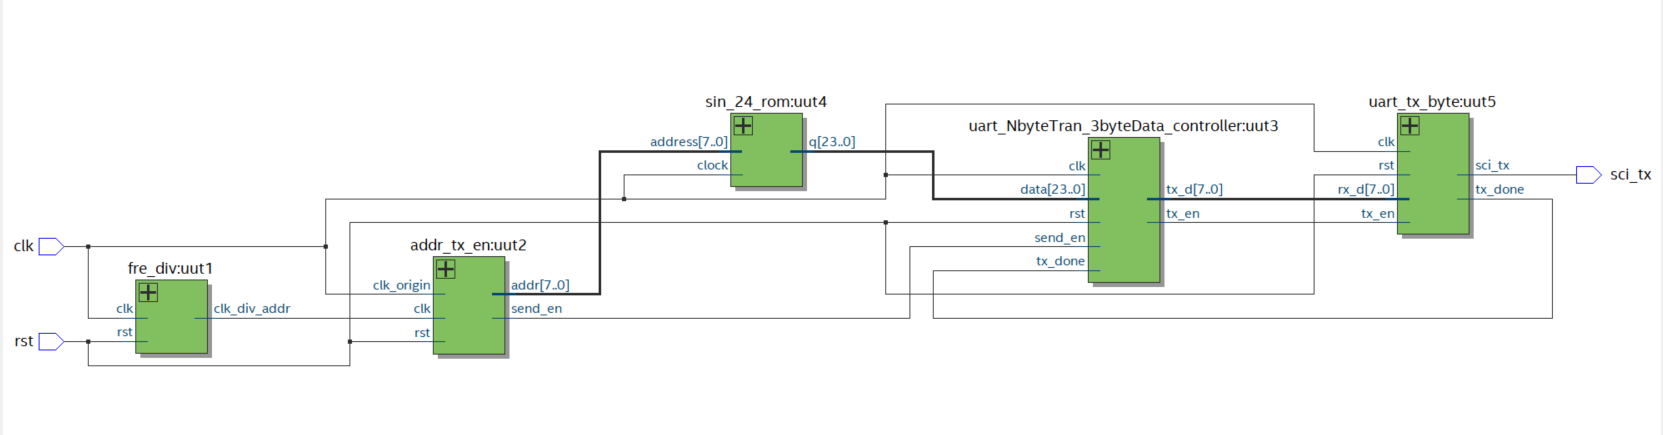
\includegraphics[width=0.8\textwidth]{task1_top_rtl.png}
    \caption{task1顶层模块RTL图}
    \label{fig:task1_top_rtl}
\end{figure}
\subsection{实验结果}
按照任务要求将simulink设置如图\ref{fig:task1_simulink}所示。接收结果如图\ref{fig:task1_result}所示,可以看出数据成功发送。
\begin{figure}[!ht]
    \centering
    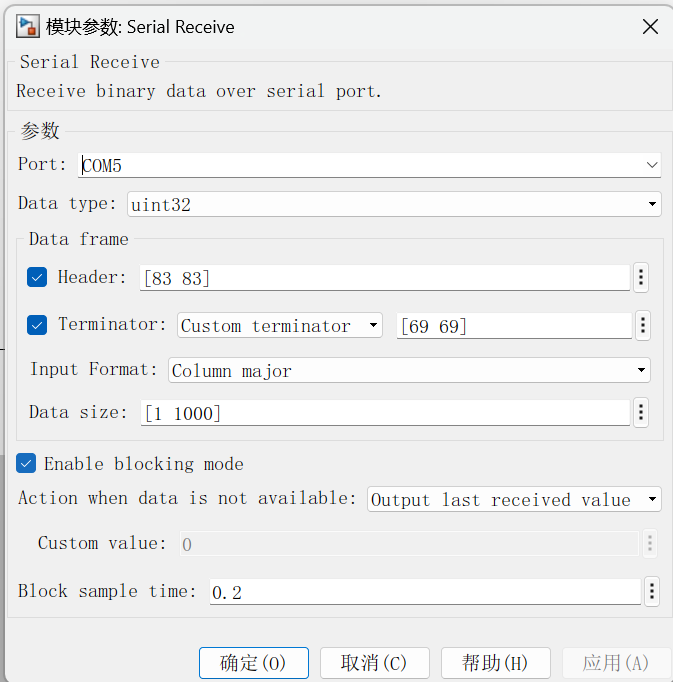
\includegraphics[width=0.8\textwidth]{task1_simulink.png}
    \caption{task1 simulink设置}
    \label{fig:task1_simulink}
\end{figure}

\begin{figure}[!ht]
    \centering
    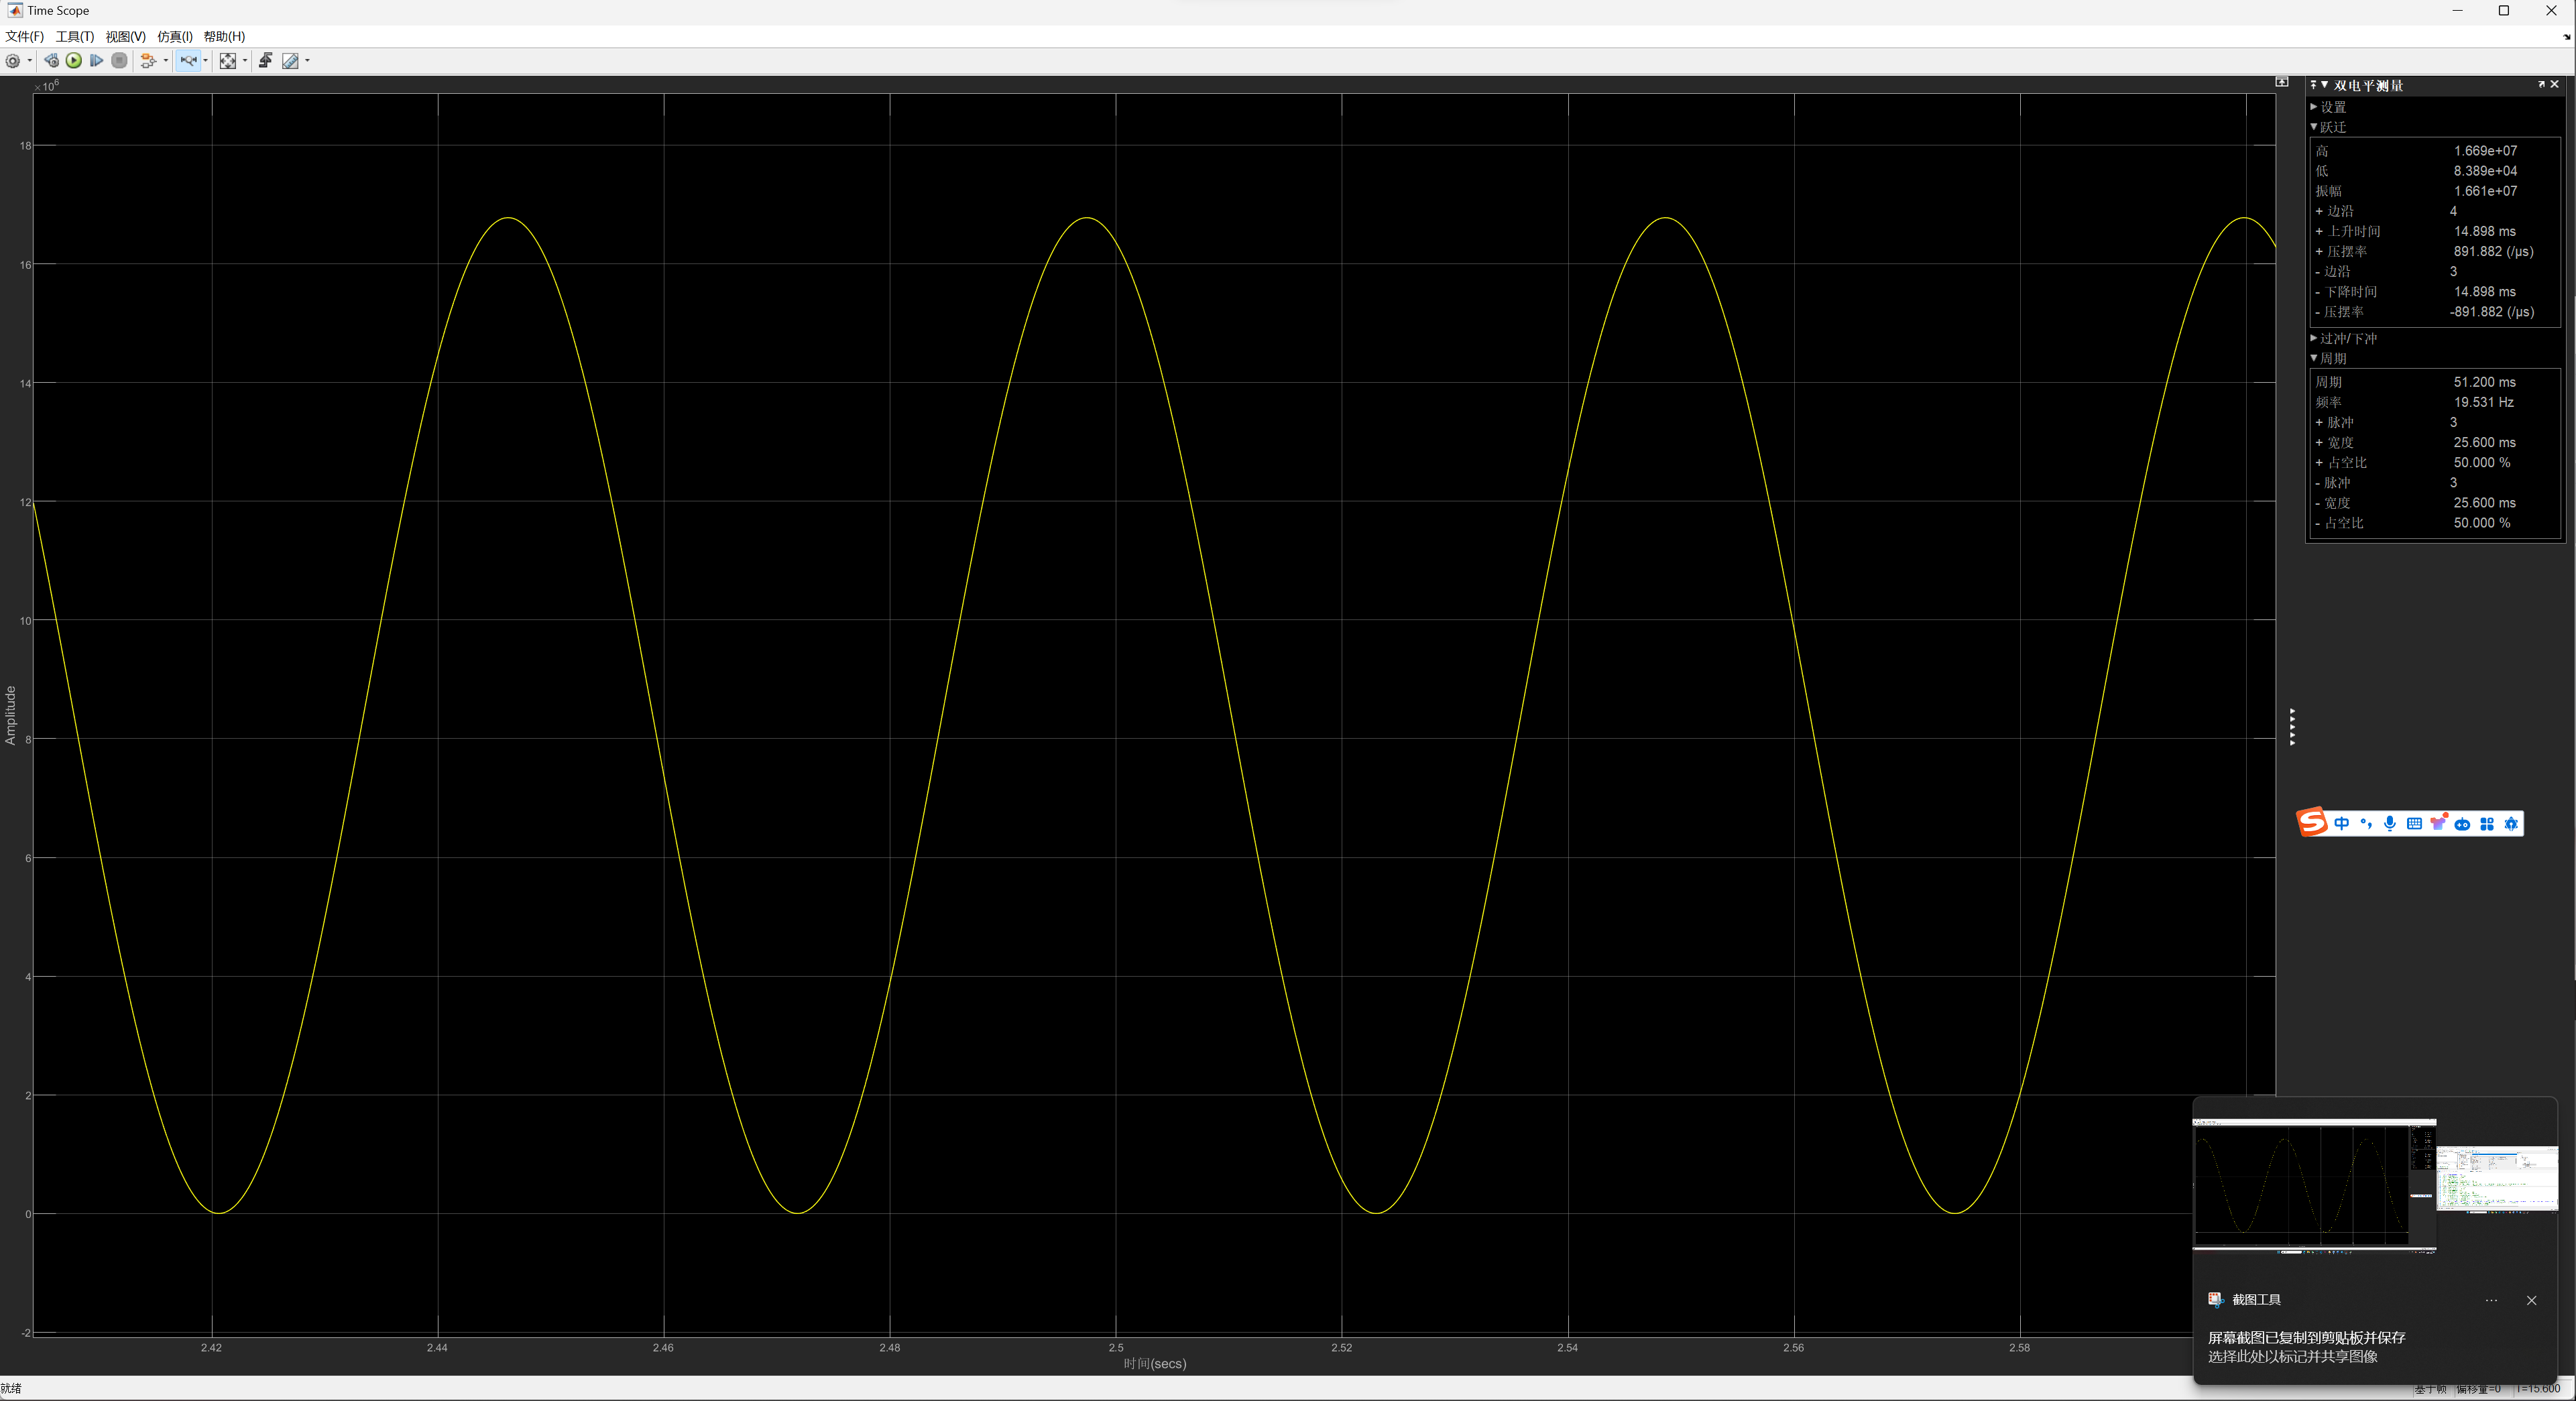
\includegraphics[width=0.8\textwidth]{task1_result.png}
    \caption{task1 接收结果}
    \label{fig:task1_result}
\end{figure}
\FloatBarrier
\section{task2}
\subsection{模块设计}
task2中使用的24位正弦波数据与task1中使用的24位正弦波数据相同,可以直接使用。
\subsubsection{地址模块}
地址模块代码如下:
\begin{framed}
    \begin{lstlisting}[style=verilogStyle]
    module rom_data_tri (
    input lr_ch_tri_clk,
    input rst,
    output reg [7:0] addr_chL,
    output reg [7:0] addr_chR
);
    always @(posedge lr_ch_tri_clk or posedge rst) begin
        if (rst) begin
            addr_chL <= 8'd0;
        end else begin
            if (addr_chL == 8'd255) begin
                addr_chL <= 8'd0;
            end else begin
                addr_chL <= addr_chL + 1'b1;
            end
        end
    end

    always @(negedge lr_ch_tri_clk or posedge rst) begin
        if (rst) begin
            addr_chR <= 8'd0;
        end else begin
            if (addr_chR >= 8'd255) begin
                addr_chR <= 8'd0;
            end else begin
                addr_chR <= addr_chR + 2'd2;
            end
        end
    end

endmodule
    \end{lstlisting}
\end{framed}
地址模块将DAC传出的lrck\_dac信号作为时钟信号,每次上升沿时,addr\_chL自增1,addr\_chR自增2。因此右通道的频率为左通道的二倍。\footnote{要想实现两路信号频率不同应该有更好的方法,但我修改时钟的方法无法实现,会产生无规律的波形}

\subsubsection{顶层模块}
顶层模块代码如下:
\begin{framed}
    \begin{lstlisting}[style=verilogStyle]
`include "rom_data_tri.v"
`include "rom_array_sync.v"
`include "dac_controller.v"
`include "fre_div.v"
module task2_top(
    input clk,
    input rst,
    output lrck_dac,
    output sclk_dac,
    output mclk_dac,
    output sdata_dac
);

wire[23:0] data_dac_chL;
wire[23:0] data_dac_chR;
wire[7:0] addr_chL;
wire[7:0] addr_chR;
wire c0;//6553600hz
wire c1;//13107200hz

rom_data_tri uut1(
    .lr_ch_tri_clk(lrck_dac),
    .rst(rst),
    .addr_chL(addr_chL),
    .addr_chR(addr_chR)
);

rom_array_sync uut2(
    .clock(clk),
    .address(addr_chL),
    .q(data_dac_chL)
);

rom_array_sync uut3(
    .clock(clk),
    .address(addr_chR),
    .q(data_dac_chR)
);

dac_controller uut4(
    .clk(c0),
    .rst(rst),
    .data_dac_chL(data_dac_chL),
    .data_dac_chR(data_dac_chR),
    .mclk_dac(mclk_dac),
    .sclk_dac(sclk_dac),
    .lrck_dac(lrck_dac),
    .sdata_dac(sdata_dac)
);

fre_div uut5(
    .inclk0(clk),
    .c0(c0)
);
endmodule
    \end{lstlisting}
\end{framed}

其中fre\_div为使用IP核生成的频率分频器,将clk分频为6553600hz作为DAC的时钟信号,从而实现DAC输出的音频信号频率为6553600hz/256/256=100\unit{Hz}。

对应的RTL图如图\ref{fig:task2_top_rtl}所示。
\begin{figure}[!ht]
    \centering
    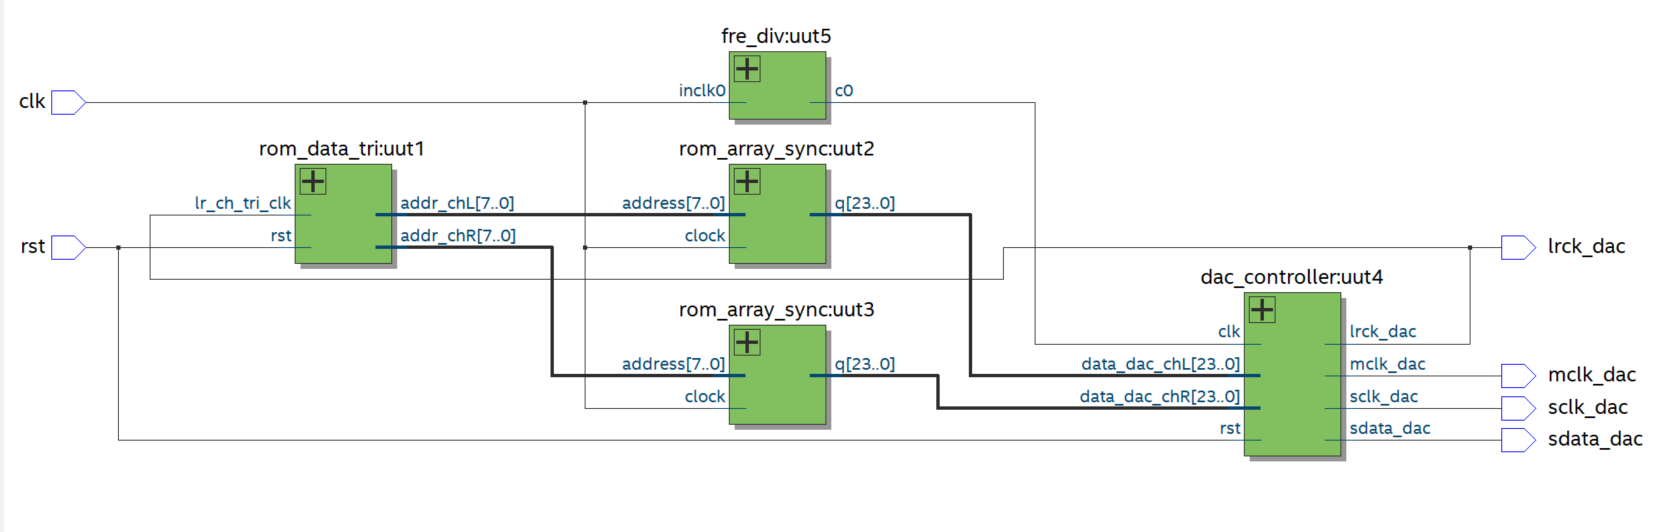
\includegraphics[width=0.8\textwidth]{task2_top_rtl.png}
    \caption{task2顶层模块RTL图}
    \label{fig:task2_top_rtl}
\end{figure}

\subsection{实验结果}
示波器测量的DAC输出信号如图\ref{fig:task2_result}所示,可以看出两路信号频率为二倍关系,一个为100\unit{Hz},一个为50\unit{Hz}。

\begin{figure}[!ht]
    \centering
    \includegraphics[width=0.8\textwidth, angle = 270]{task2_result.png}
    \caption{task2 DAC输出信号}
    \label{fig:task2_result}
\end{figure}
\end{document}